\documentclass[a4paper]{article}

\input{../_auxiliary/preamble/1_preamble_functionality_main.tex}
\input{../_auxiliary/preamble/2_preamble_layout_report.tex}

\usepackage[
    backend=biber,
    style=ieee
]{biblatex}
\addbibresource{references.bib}
\input{../_auxiliary/preamble/1_preamble_functionality_bibliography.tex}

\input{../_auxiliary/preamble/4_preamble_tikz_symbols}

\renewcommand{\contentsname}{\centering Contents} % https://tex.stackexchange.com/a/308207
\usepackage[titles, subfigure]{tocloft} % https://tex.stackexchange.com/a/336618
\renewcommand{\cftsecleader}{\cftdotfill{\cftdotsep}} % https://tex.stackexchange.com/a/271942

%%%%%%%%%%%%%%%%%%%%%%%%%%%%%%%%%%%%%%%%%%%%%%%%%%%%%%%%%%%%%%%%%%%%%

\begin{document}

\section*{Welcome Letter}
\label{sec:abstract}

\begin{minipage}{0.6\textwidth}

Dear Academy participants, \\

we look forward to welcoming you to our Summer Academy! \\

We live in a time of unprecedented global construction activity. All major urban regions are experiencing strong growth. The construction sector is now responsible for more than 40\% of annual global carbon emissions. Since the majority of construction-related emissions are hard to abate, this number is expected to grow for the foreseeable future. Despite the urgency of reducing carbon emissions, new buildings are often designed with a service life of around 50 years only. At the same time, a growing number of opinion polls point toward a deep-rooted dissatisfaction among the general population with the modernist style in which the majority of buildings is now designed. This is supported by a number of recent neuro-scientific experiments. \\

This disconnect between the taste of architects and the general public is by no means a novel phenomenon and has been widely caricatured, as illustrated in the sketch by Raymond Loewy shown on the right. However, recent work by contemporary philosophers, including Sir Roger Scruton \textit{"Why Beauty Matters"} and Alain de Botton \textit{"Why is the Modern World So Ugly?"} have re-invigorated public debate. \\

In light of these developments, cognitive scientists, citizen initiatives and a select group of architects and designers have pointed to elements of traditional architecture as a tangible remedy to the featureless façades that have come to dominate real estate projects in recent decades. \\

During this Summer Academy, we are hosting a group of speakers that, through their academic or professional work, are shaping the current conversation around architecture, beauty and nature. \\ 

As participants of the Academy, you will learn why architects came to believe that \textit{béton brut} was the material of the future, if and how we can ever hope to quantify the aesthetics of a building, what the real environmental footprint of modern construction is, and how citizen action can help shape the built environment $\dots$ and so much more. \\

See you soon - all the best!
\textit{Michael, Philippe and Mark}

\end{minipage}\hspace{15mm}
\begin{minipage}{0.325\textwidth}
    \begin{figure}[H]
    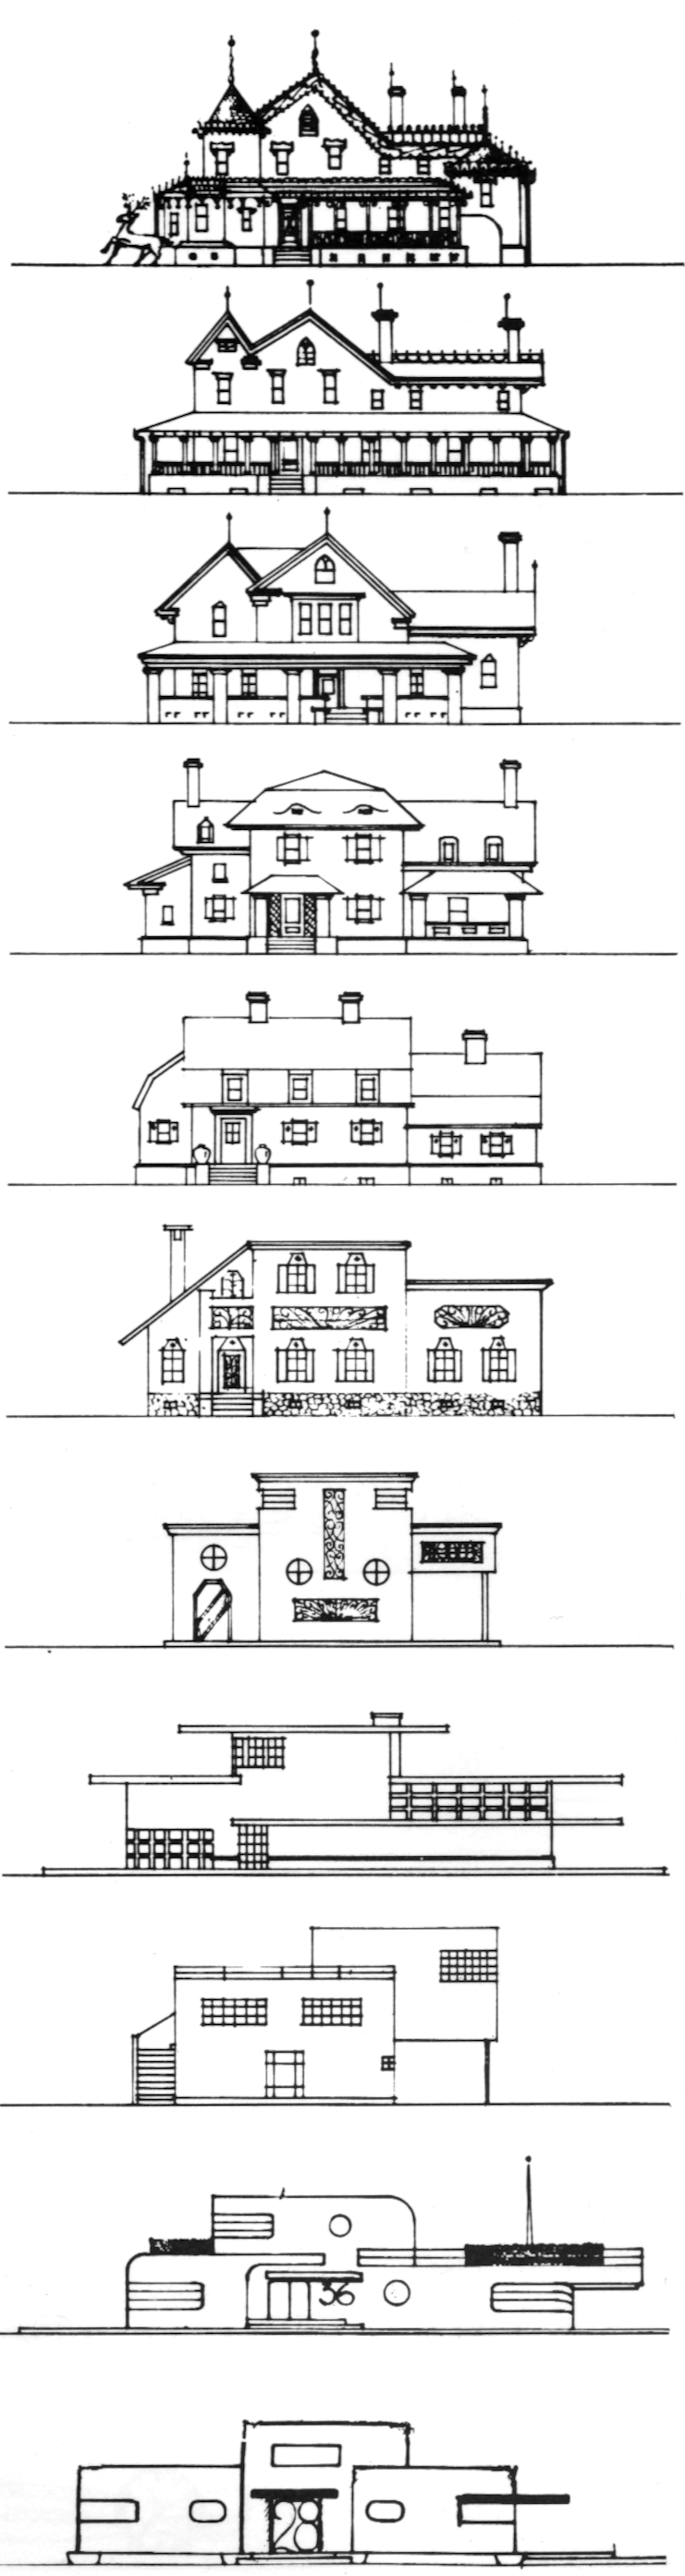
\includegraphics[width=50mm]{../1_proposal/figures/loewy_architecture.png}
    \label{fig:loewy}
    \end{figure}
\end{minipage}

\clearpage

\section*{About the Academy Organizers}

\textbf{\textit{Michael P. Weinold}} (born 1995 in Innsbruck, Austria) is a doctoral researcher at ETH Zurich and the Paul Scherrer Institute. His background is in engineering physics, with degrees from Vienna University of Technology and ETH Zurich. His current research is focused on accelerating innovation in novel clean-energy technologies. He builds mathematical models and open-source software to better help decision makers assess the environmental impact of different techno-economic scenarios for decarbonizing the economy. Since 2023, he is a guest lecturer at the Department of Mechanical Engineering of ETH Zurich. His interest in aesthetics in the built environment was sparked during his research at the University of Cambridge, where he was introduced to the legacy of the late British philosopher Sir Roger Scruton. Since that time, he has been most interested in how new neuro-scientific insights can enable citizen movements to positively shape public spaces.

\textbf{\textit{Philippe Schultheiss}} (born 1984 in Basel, Switzerland) is a consultant and soon-to-be pastor in the Swiss Reformed Church. He holds undergraduate degrees in Business \& Economics from the university of Basel as well as a master's degree in Medieval Philosophy from the university of Freiburg i.Ue. He is now an alumnus of the Swiss Study Foundation, where he is still active as a member of the Assessment Jury as well as a frequent host of events. He has been interested in politics, especially the areas of environmental and urban planning, since his days at the cantonal school at Schaffhausen. He went on to co-found the Green-Liberal Party in his home canton and remained involved in local politics after his relocation to Zurich, where, in 2020, he was elected president of the Parliament of the Reformed Church Zurich. This community of more than 70'000 members administers dozens of church buildings. Hence his motivation to contribute to a prospective and socially beneficial real estate strategy.

\textbf{\textit{Mark C. Ballandies}} (born 1991 in Burgwedel, Germany) is a postdoctoral researcher in the Computational Social Science group at ETH Zurich, where he is exploring decentralised, bottom-up and community-owned solutions to complex societal challenges. In addition, he is involved in the startup WiHi that uses a decentralized network of stations to improve weather and climate predictions. He is the co-founder of DAOSuisse, a lecturer at the Vorarlberg University of Applied Sciences, an alumnus of the Foundation of German Business, president of education matters e.V. and initiator of the Smarte Dörfer association. In 2019, Mark discovered the beauty of old farmhouses and their effectiveness in combating environmental challenges when he began restoring a half-timbered house in his home village, using ecological, locally sourced and recyclable building materials such as wood, clay and hemp. He found that these farmhouses integrate values such as circularity, sustainability and locality into all aspects and details of their design and construction, resulting in unique, sustainable and liveable architecture. This discovery inspires him in his daily work, which he enjoys sharing with others.

\end{document}